This section shows the measurements obtained with the TRITIUM-IFIC 0 prototype during its installation in the IFIC laboratory.

As stated above, a statistically significant number of events was not obtained when the prototype was read by two PMTs in coincidence. To overcome this problem, a single PMT measurement was taken using the electronic chain configuration shown in figure \ref{subfig:ElectronicConfiguraiton1PMT}. The energy spectra were measured for both, the signal and background prototypes, which are shown in Figure \ref{subfig:SignalBackgroundEnergySpectraTritiumIFIC0}. As reported above, the signal prototype was filled with a tritiated water solution of $99.696~\kilo\becquerel/\liter$ activity and the background prototype was filled with ultrapure water. A difference between signal and background, Figure \ref{subfig:TritiumEnergySpectraTritiumIFIC0}, corresponds to the energy spectrum of tritium. The number of counts per second obtained for the three spectra is given in Table \ref{tab:CountsPerSecondTRITIUMIFIC0}, where the tritium counts are obtained from the difference of signal and backgorund.


\begin{figure}
\centering
    \begin{subfigure}[b]{1\textwidth}
    \centering
    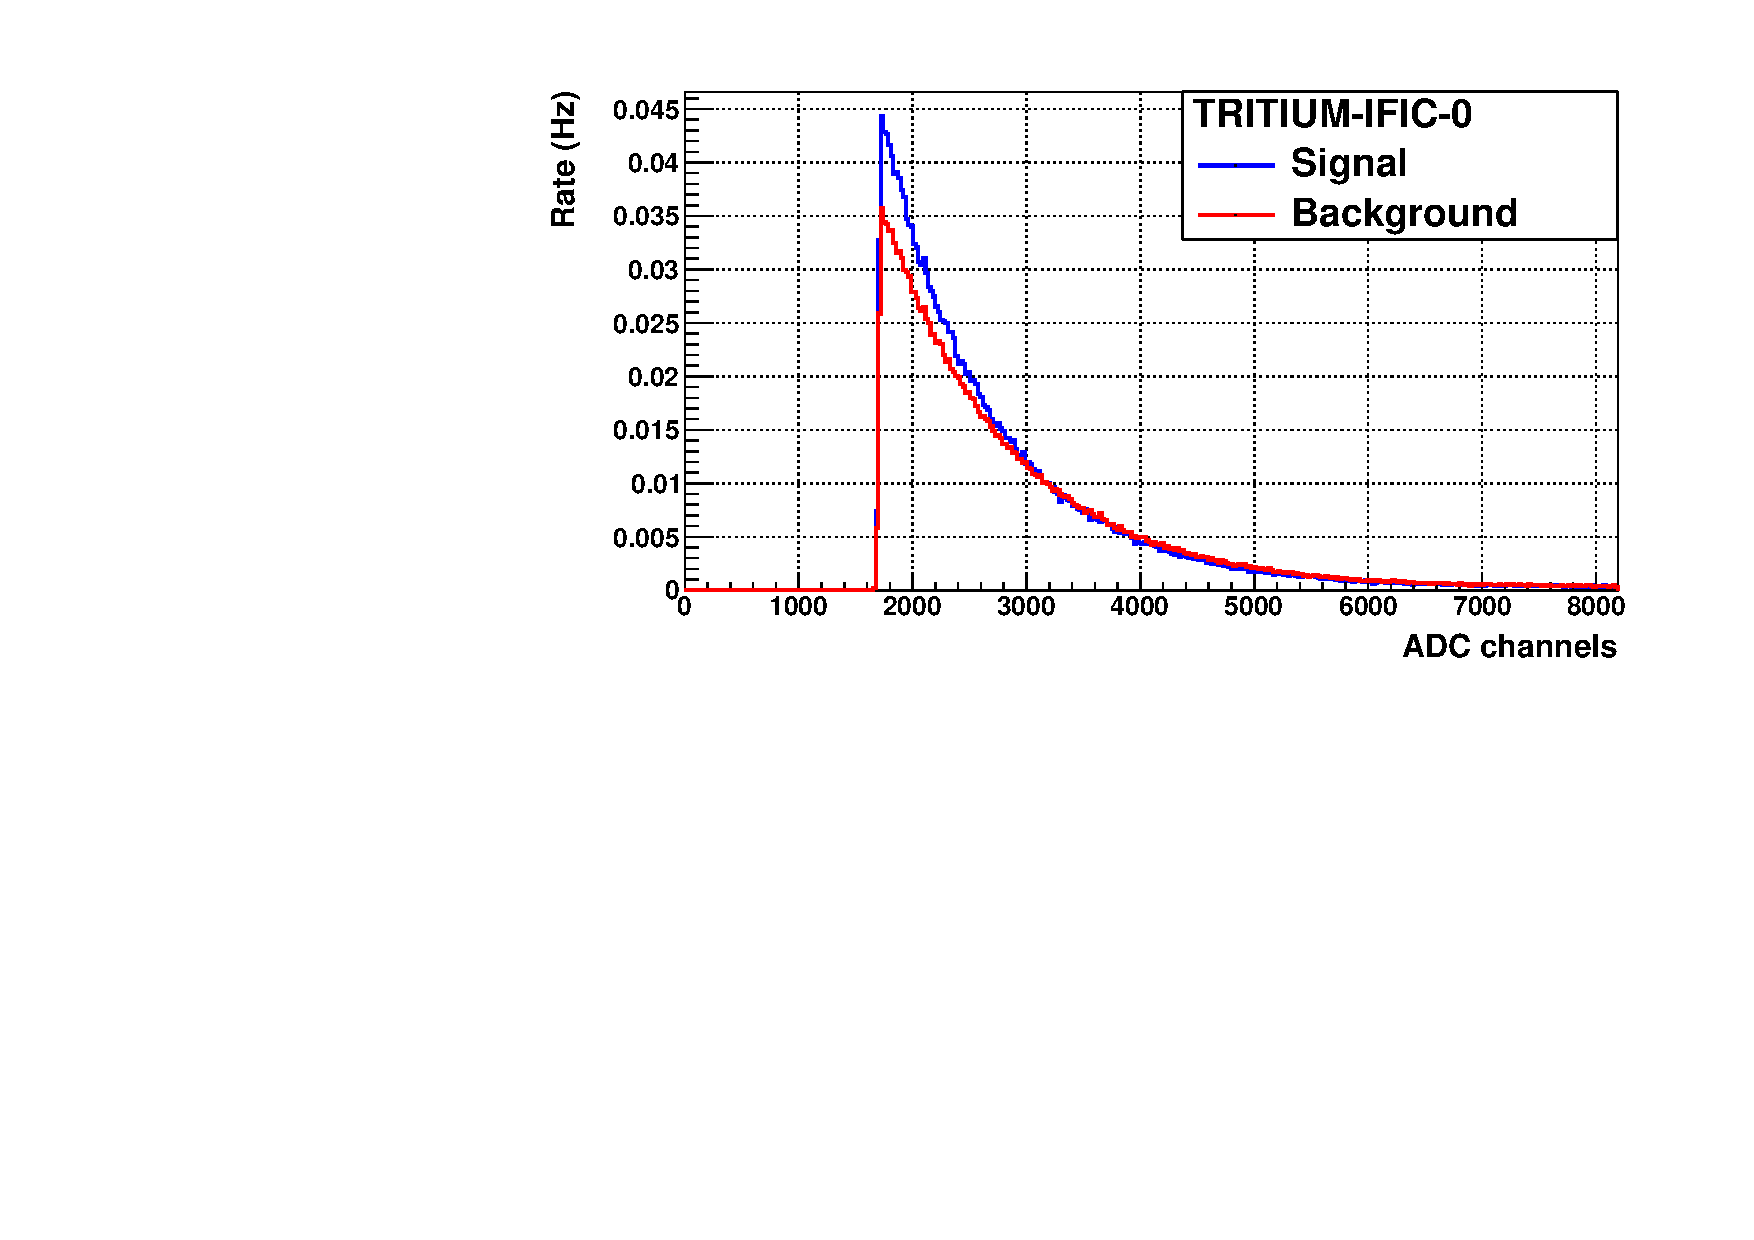
\includegraphics[width=\textwidth]{7ExperimentalResultsDetectors/71ExperimentalResultsLaboratory/711TritiumIFIC0/TritiumIFIC0Signals.pdf}  
    \caption{.\label{subfig:SignalBackgroundEnergySpectraTritiumIFIC0}}
    \end{subfigure}
    \hfill
    \begin{subfigure}[b]{1\textwidth}
    \centering
    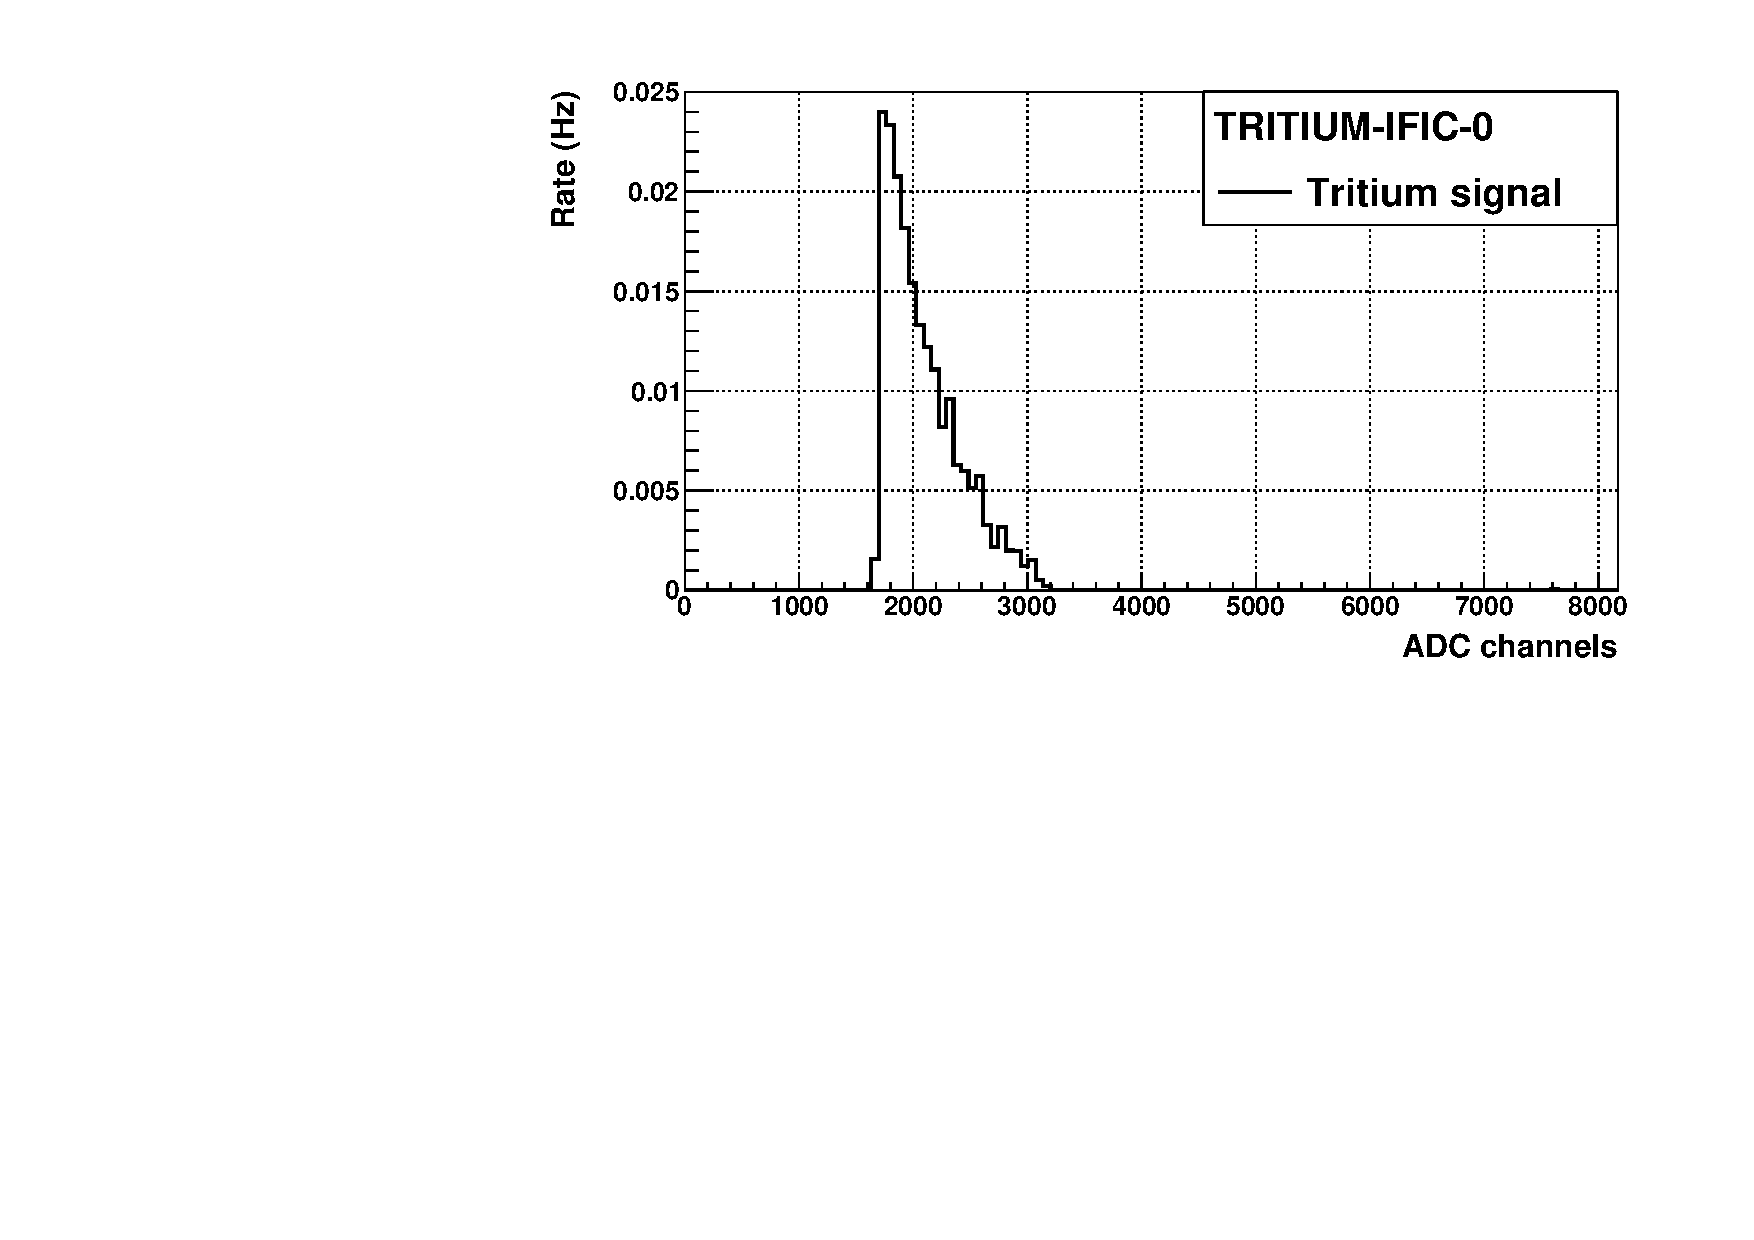
\includegraphics[width=\textwidth]{7ExperimentalResultsDetectors/71ExperimentalResultsLaboratory/711TritiumIFIC0/TritiumIFIC0ClearRebin.pdf}  
    \caption{\label{subfig:TritiumEnergySpectraTritiumIFIC0}}
    \end{subfigure}
 \caption{Energy spectra measured with TRITIUM-IFIC 0 prototype. a) Signal and background energy spectra. b) Tritium energy spectrum.}
 \label{fig:EnergySpectraTRITIUMIFIC0}
\end{figure}

\begin{table}[htbp]
\centering{}%
\begin{tabular}{cc}
\toprule 
Spectrum & Counts/second \tabularnewline
\midrule
\midrule 
Signal prototype & $2.27 \pm 0.06$ \tabularnewline
Background prototype & $2.06 \pm 0.06$ \tabularnewline  
Tritium counts & $0.21 \pm 0.085$ \tabularnewline
\bottomrule
\end{tabular}
\caption{Counting rate obtained with the TRITIUM-IFIC 0 prototype.}
\label{tab:CountsPerSecondTRITIUMIFIC0}
\end{table}

The tritium detection efficiency obtained for this prototype is $(2.11 \pm 0.85)\cdot{} 10^{-3}~\liter\second^{-1}\kilo\becquerel^{-1}$, calculated from the ratio of both, the tritium counting rate measured and the specific activity of the tritium liquid source. 

As we reported in section \ref{sec:StateOfTheArt}, the efficiency of scintillating detectors scales with the active area of the scintillator used. Therefore, to compare the efficiency with oher detectors and with other prototypes developed in TRITIUM experiment, the specific efficiency of this prototype is calculated by normalizing to the scintillator area, which is $(9.59 \pm 3.88)\cdot{} 10^{-6}~\liter\second^{-1}\kilo\becquerel^{-1}\cm^{-2}$. As can be seen in Table \ref{tab:PlasticScinTritium}, the specific efficiency is a somewhat larger than that obtained for Muramatsu and Moghissi \cite{Moghissi}, which is a low efficiency. This fact can be explained by the loss of photons in the curve of the fiber bunch, as demostrated in section above.